% !Mode:: "TeX:UTF-8"
\chapter{数学公式的输入方法}
湖南师范大学研究生论文有关公式、数字、年代、符号的书写要求:
\begin{itemize}
	\item 年份一概写全数。例:1998年不能写成98年。
	\item 分数、世纪、年代均以阿拉伯数字表示。例:三分之二写成2/3;二十世纪九十年代写成20世纪90年代。
	\item 公式均需标注公式号,公式号用圆括号,阿拉伯数字表示,按章编排。
	\item 论文中的物理量、量纲及符号等均采用国际标准(SI)和国家标准(GB)。
\end{itemize}
\section{研究生毕业设计论文的公式规范}
论文中的公式应另起行,原则上应居中书写,与周围文字留有足够的空间区分开。
若公式前有文字(如“解”、“假定”等),文字空两格写,公式仍居中写。公式末不加标点。

公式应标注序号,并将序号置于括号内。 公式序号按章编排,如第1章第一个公式序号为“(1-1)”。公式的序号右端对齐。

公式较长时最好在等号“=”处转行,如难实现,则可在$+$、$-$、$\times$、$\div$运算符号处转行,转行时运算符号仅书写于转行式前,不重复书写。

文中引用公式时,一般用“见式(1-1)”或“由公式(1-1)”。

公式中用斜线表示“除”的关系时应采用括号,以免含糊不清,如$a/(b\cos x)$。通常“乘”的关系在前,如$a\cos x/b$而不写成$(a/b)\cos x$。

不能用文字形式表示等式,如:$\textnormal{刚度}=\frac{{\textnormal{受力}}}{{\textnormal{受力方向的位移}}}$。

对于数学公式的输入方法,网络上有一个比较全面权威的文档{\bf{\href{http://tug.ctan.org/cgi-bin/ctanPackageInformation.py?id=voss-mathmode}{Math mode}}}请大家事先大概浏览一下。下面将对学位论文中主要用到的数学公式排版形式进行阐述。

\section{生成\LaTeX~数学公式的两种方法}
对于先前没有接触过\LaTeX~的人来说,编写\LaTeX~数学公式是一件很繁琐的事,尤其是对复杂的数学公式来说,更可以说是一件难以完成的任务。
实际上,生成\LaTeX~数学公式有两种较为简便的方法,一种是基于MathType数学公式编辑器的方法,另一种是基于MATLAB商业数学软件的方法,
下面将分别对这两种数学公式的生成方法作一下简单介绍。

\subsection{基于MathType软件的数学公式生成方法}
MathType是一款功能强大的数学公式编辑器软件,能够用来在文本环境中插入Windows OLE图形格式的复杂数学公式,所以应用比较普遍。但此软件只有30天的试用期,之后若再继续使用则需要付费购买才行。网络上有很多破解版的MathType软件可供下载免费使用,
笔者推荐下载安装版本号在6.5之上的中文破解版。

在安装好MathType之后,若在输入窗口中编写数学公式,复制到剪贴板上的仍然是图形格式的对象。
若希望得到可插入到\LaTeX~编辑器中的文本格式对象,则需要对MathType软件做一下简单的设置:在MathType最上排的按钮中依次选择“参数选项
$\to$转换”,在弹出的对话窗中选中“转换到其它语言(文字):”,在转换下拉框中选择“Tex——LaTeX 2.09 and later”,并将对话框最下方的两个复选框全部勾掉,点击确定,这样,再从输入窗口中复制出来的对象就是文本格式的了,就可以直接将其粘贴到\LaTeX~
编辑器中了。按照这种方法生成的数学公式两端分别有标记\verb|\[|和标记\verb|\]|,在这两个标记之间才是真正的数学公式代码。

若希望从MathType输入窗口中复制出来的对象为图形格式,则只需再选中“公示对象(Windows OLE图形)”即可。

\subsection{基于MATLAB软件的数学公式生成方法}
MATLAB是矩阵实验室(Matrix Laboratory)的简称,是美国MathWorks公司出品的商业数学软件。它是当今科研领域最常用的应用软件之一,
具有强大的矩阵计算、符号运算和数据可视化功能,是一种简单易用、可扩展的系统开发环境和平台。

MATLAB中提供了一个latex函数,它可将符号表达式转化为\LaTeX~数学公式的形式。其语法形式为latex(s),其中,s为符号表达式,
之后再将latex函数的运算结果直接粘贴到\LaTeX~编辑器中。从\LaTeX~数学公式中可以发现,其中可能包含如下符号组合:

\vspace{1em}\noindent\hrule

\begin{verbatim*}
	\qquad=两个空铅(quad)宽度
	\quad=一个空铅宽度
	\;=5/18空铅宽度
	\:=4/18空铅宽度
	\,=3/18空铅宽度
	\!=-3/18空铅宽度
	\ =一个空格
\end{verbatim*}

\noindent\hrule\vspace{1em}

所以最好将上述符号组合从数学公式中删除,从而使数学公式显得匀称美观。

对于Word等软件的使用者来说,在我们通过MATLAB运算得到符号表达式形式的运算结果时,在Word中插入运算结果需要借助于MathType软件,
通过在MathType中输入和MATLAB运算结果相对应的数学表达形式,之后再将MathType数学表达式转换为图形格式粘贴到Word中。实际上,
也可以将MATLAB中采用latex函数运行的结果直接粘贴到MathType中,再继续上述步骤,这样可以大大节省输入公式所需要的时间。
此方法在MathType6.5c上验证通过,若您粘入到MathType中的仍然为从MATLAB中导入的代码,请您更新MathType软件。

\section{数学字体}
在数学模式下,常用的数学字体命令有如下几种:

\vspace{1em}\noindent\hrule
\begin{verbatim}
	\mathnormal或无命令 用数学字体打印文本;
	\mathit             用斜体(\itshape)打印文本;
	\mathbf             用粗体(\bfseries)打印文本;
	\mathrm             用罗马体(\rmfamily)打印文本;
	\mathsf             用无衬线字体(\sffamily)打印文本;
	\mathtt             用打印机字体(\ttfamily)打印文本;
	\mathcal            用书写体打印文本;
\end{verbatim}
\noindent\hrule\vspace{1em}

在学位论文撰写中,只需要用到上面提到的\verb|\mathit|、\verb|\mathbf|和\verb|\mathrm|命令。若要得到Times New Roman的数学字体,则需要调用txfonts宏包(此宏包实际上采用的是Nimbus Roman No9 L字体,
它是开源系统中使用的免费字体,其字符字体与Times New Roman字体几乎完全相同);若要得到粗体数学字体,则需要调用bm宏包。表\ref{tab:fonts}中分别列出了得到阿拉伯数字、拉丁字母和希腊字母
各种数学字体的命令。

\begin{table}[htbp]
	\caption{常用数学字体命令一览}\label{tab:fonts}
	\vspace{0.5em}\centering\zihao{5}
	\begin{tabular}{llll}
		\toprule
		       & 阿拉伯数字\&大写希腊字母 & 大小写拉丁字母          & 小写希腊字母            \\
		\midrule
		斜体   & \verb|\mathit{}|   & \verb|无命令|  & \verb|无命令|  \\
		粗斜体 & \verb|\bm{\mathit{}}|   & \verb|\bm{}| & \verb|\bm{}| \\
		直立体 & \verb|无命令|  & \verb|\mathrm{}| & \verb|字母后加up| \\
		粗体   & \verb|\mathbf{}或\bm{}|  & \verb|\mathbf{}| & \verb|\bm{字母后加up}| \\
		\bottomrule
	\end{tabular}
	\vspace{\baselineskip}
\end{table}

\noindent 下面列出了一些应采用直立数学字体的数学常数和数学符号。

\vspace{-0.5em}
\begin{center}
	\begin{tabularx}{0.9\textwidth}{XX}
		$\mathrm{d}$、 $\mathrm{D}$、 $\mathrm{p}$———微分算子 & $\mathrm{e}$———自然对数之底数 \\
		$\mathrm{i}$、 $\mathrm{j}$———虚数单位                & $\piup$———圆周率               \\
	\end{tabularx}
\end{center}

\section{行内公式}
出现在正文一行之内的公式称为行内公式,例如$f(x)=\int_{a}^{b}\frac{\sin{x}}{x}\mathrm{d}x$。对于非矩阵和非多行形式的行内公式,一般不会使得行距发生变化,而Word等软件却会根据行内公式的竖直距离而自动调节行距,如图\ref{fig:hangju}所示。

\begin{figure}[htbp]
	\centering
	\subfigure[由\LaTeX~系统生成的行内公式]{\label{fig:subfig:latex}
		\fbox{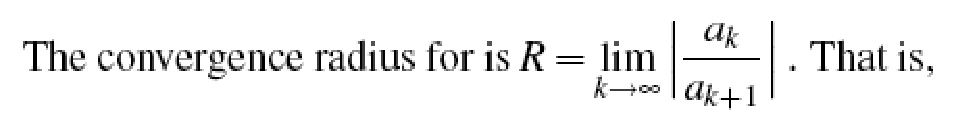
\includegraphics[width=0.55\textwidth]{latex}}}
	\subfigure[由Word软件生成的.doc格式行内公式]{\label{fig:subfig:word}
		\fbox{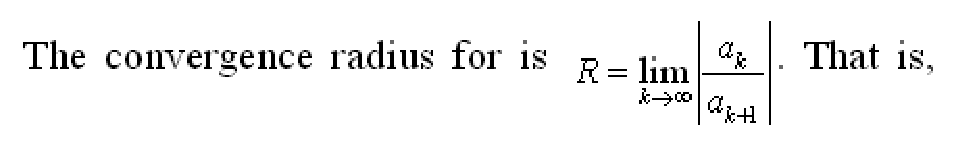
\includegraphics[width=0.55\textwidth]{word}}}
	\subfigure[由Word软件生成的.pdf格式行内公式]{\label{fig:subfig:pdf}
		\fbox{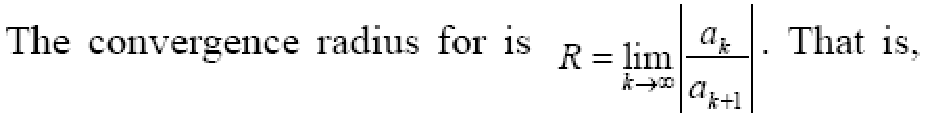
\includegraphics[width=0.55\textwidth]{pdf}}}

	\caption{由\LaTeX~和Word生成的3种行内公式屏显效果}\label{fig:hangju}
	\vspace{-1em}
\end{figure}

这三幅图分别为\LaTeX~和Word生成的行内公式屏显效果,从图中可看出,在\LaTeX~文本含有公式的行内,在正文与公式之间对接工整,行距不变;而在Word文本含有公式的行内,在正文与公式之间对接不齐,行距变大。因此从这一点来说,
\LaTeX~系统在数学公式的排版上具有很大优势。

\LaTeX~提供的行内公式最简单、最有效的方法是采用\TeX~本来的标记———开始和结束标记都写作\$,例如本段开始的例子可由下面的输入得到。
\verb|$f(x)=\int_{a}^{b}\frac{\sin{x}}{x}\mathrm{d}x$|

\section{行间公式}
位于两行之间的公式称为行间公式,每个公式都是一个单独的段落,例如
\[\int_a^b{f\left(x\right)\mathrm{d}x}=\lim_{\left\|\Delta{x_i}\right\|\to 0}\sum_i{f\left(\xi_i\right)\Delta{x_i}}\]
除人工编号外,\LaTeX~各种类型行间公式的标记见表\ref{tab:eqtag}。
\begin{table}[htbp]
	\caption{各种类型行间公式的标记}\label{tab:eqtag}
	\vspace{0.5em}\centering\zihao{5}
	\begin{tabularx}{\textwidth}{cll}
		\toprule
		         & 无编号                     & 自动编号                \\
		\midrule
		单行公式 & \verb|\begin{displaymath}... \end{displaymath}|    & \verb|\begin{equation}... \end{equation}| \\
		         & 或\verb|\[...\]| &                         \\
		多行公式 & \verb|\begin{eqnarray*}... \end{eqnarray*}|    & \verb|\begin{eqnarray}... \end{eqnarray}| \\
		\bottomrule
	\end{tabularx}
\end{table}

另外,在自动编号的某行公式行尾添加标签\verb|\nonumber|,可将该行转换为无编号形式。

行间多行公式需采用\verb|eqnarray|或\verb|eqnarray*|环境,它默认是一个列格式为\verb|rcl|的3列矩阵,并且中间列的字号要小一些,因此通常只将需要对齐的运算符号(通常为等号“=”)置于中间列。

\section{可自动调整大小的定界符}
若在左右两个定界符之前分别添加命令\verb|\left|和\verb|\right|,则定界符可根据所包围公式大小自动调整其尺寸,这可从式(\ref{nodelimiter})和式(\ref{delimiter})中看出。
\begin{equation}\label{nodelimiter}
	(\sum_{k=\frac12}^{N^2})
\end{equation}
\begin{equation}\label{delimiter}
	\left(\sum_{k=\frac12}^{N^2}\right)
\end{equation}
式(\ref{nodelimiter})和式(\ref{delimiter})是在\LaTeX~中分别输入如下代码得到的。
\begin{verbatim}
	(\sum_{k=\frac12}^{N^2})
	\left(\sum_{k=\frac12}^{N^2}\right)
\end{verbatim}
\verb|\left|和\verb|\right|总是成对出现的,若只需在公式一侧有可自动调整大小的定界符,则只要用“.”代替另一侧那个无需打印出来的定界符即可。

若想获得关于此部分内容的更多信息,可参见\href{http://tug.ctan.org/cgi-bin/ctanPackageInformation.py?id=voss-mathmode}{Math mode}文档的第8章“Brackets, braces and parentheses”。

\section{数学重音符号}
数学重音符号通常用来区分同一字母表示的不同变量,输入方法如下(需要调用\verb|amsmath|宏包):

\vspace{0.5em}\noindent\zihao{5}\begin{tabularx}{\textwidth}{Xc|Xc|Xc}
	\verb|\acute| & $\acute{a}$ & \verb|\mathring| & $\mathring{a}$           & \verb|\underbrace| & $\underbrace{a}$          \\
	\verb|\bar| & $\bar{a}$   & \verb|\overbrace| & $\overbrace{a}$          & \verb|\underleftarrow| & $\underleftarrow{a}$      \\
	\verb|\breve| & $\breve{a}$ & \verb|\overleftarrow| & $\overleftarrow{a}$      & \verb|\underleftrightarrow| & $\underleftrightarrow{a}$ \\
	\verb|\check| & $\check{a}$ & \verb|\overleftrightarrow| & $\overleftrightarrow{a}$ & \verb|\underline| & $\underline{a}$           \\
	\verb|\dddot| & $\dddot{a}$ & \verb|\overline| & $\overline{a}$           & \verb|\underrightarrow| & $\underrightarrow{a}$     \\
	\verb|\ddot| & $\ddot{a}$  & \verb|\overrightarrow| & $\overrightarrow{a}$     & \verb|\vec| & $\vec{a}$                 \\
	\verb|\dot| & $\dot{a}$   & \verb|\tilde| & $\tilde{a}$              & \verb|\widehat| & $\widehat{a}$             \\
	\verb|\grave| & $\grave{a}$ & \verb|\underbar| & $\underbar{a}$           & \verb|\widetilde| & $\widetilde{a}$           \\
	\verb|\hat| & $\hat{a}$
\end{tabularx}\vspace{0.5em}
\zihao{4} 当需要在字母$i$和$j$的上方添加重音符号时,为了去掉这两个字母顶上的小点,这两个字母应该分别改用\verb|\imath|和\verb|\jmath|。

如果遇到某些符号不知道该采用什么命令能输出它时,则可通过\href{http://detexify.kirelabs.org/classify.html}{Detexify$^2$网站}来获取符号命令。若用鼠标左键在此网页的方框区域内画出你所要找的符号形状,则会在网页右方列出和你所画符号形状相近的5个符号及其相对应的\LaTeX~输入命令。若所列出的符号中不包括你所要找的符号,还可通过点击“Select from the complete list!”以得分从低到高的顺序列出所有符号及其相对应的\LaTeX~输入命令。

最后,建议大家还以\href{http://tug.ctan.org/cgi-bin/ctanPackageInformation.py?id=voss-mathmode}{Math mode}这篇pdf文档作为主要参考。若要获得最为标准、美观的数学公式排版形式,可以查查文档中是否有和你所要的排版形式相同或相近的代码段,通过修改代码段以获得你所要的数学公式排版形式。

